% Options for packages loaded elsewhere
\PassOptionsToPackage{unicode}{hyperref}
\PassOptionsToPackage{hyphens}{url}
%
\documentclass[
]{book}
\usepackage{amsmath,amssymb}
\usepackage{iftex}
\ifPDFTeX
  \usepackage[T1]{fontenc}
  \usepackage[utf8]{inputenc}
  \usepackage{textcomp} % provide euro and other symbols
\else % if luatex or xetex
  \usepackage{unicode-math} % this also loads fontspec
  \defaultfontfeatures{Scale=MatchLowercase}
  \defaultfontfeatures[\rmfamily]{Ligatures=TeX,Scale=1}
\fi
\usepackage{lmodern}
\ifPDFTeX\else
  % xetex/luatex font selection
\fi
% Use upquote if available, for straight quotes in verbatim environments
\IfFileExists{upquote.sty}{\usepackage{upquote}}{}
\IfFileExists{microtype.sty}{% use microtype if available
  \usepackage[]{microtype}
  \UseMicrotypeSet[protrusion]{basicmath} % disable protrusion for tt fonts
}{}
\makeatletter
\@ifundefined{KOMAClassName}{% if non-KOMA class
  \IfFileExists{parskip.sty}{%
    \usepackage{parskip}
  }{% else
    \setlength{\parindent}{0pt}
    \setlength{\parskip}{6pt plus 2pt minus 1pt}}
}{% if KOMA class
  \KOMAoptions{parskip=half}}
\makeatother
\usepackage{xcolor}
\usepackage{longtable,booktabs,array}
\usepackage{calc} % for calculating minipage widths
% Correct order of tables after \paragraph or \subparagraph
\usepackage{etoolbox}
\makeatletter
\patchcmd\longtable{\par}{\if@noskipsec\mbox{}\fi\par}{}{}
\makeatother
% Allow footnotes in longtable head/foot
\IfFileExists{footnotehyper.sty}{\usepackage{footnotehyper}}{\usepackage{footnote}}
\makesavenoteenv{longtable}
\usepackage{graphicx}
\makeatletter
\def\maxwidth{\ifdim\Gin@nat@width>\linewidth\linewidth\else\Gin@nat@width\fi}
\def\maxheight{\ifdim\Gin@nat@height>\textheight\textheight\else\Gin@nat@height\fi}
\makeatother
% Scale images if necessary, so that they will not overflow the page
% margins by default, and it is still possible to overwrite the defaults
% using explicit options in \includegraphics[width, height, ...]{}
\setkeys{Gin}{width=\maxwidth,height=\maxheight,keepaspectratio}
% Set default figure placement to htbp
\makeatletter
\def\fps@figure{htbp}
\makeatother
\setlength{\emergencystretch}{3em} % prevent overfull lines
\providecommand{\tightlist}{%
  \setlength{\itemsep}{0pt}\setlength{\parskip}{0pt}}
\setcounter{secnumdepth}{5}
\usepackage{booktabs}
\usepackage{amsthm}
\makeatletter
\def\thm@space@setup{%
  \thm@preskip=8pt plus 2pt minus 4pt
  \thm@postskip=\thm@preskip
}
\makeatother
\ifLuaTeX
  \usepackage{selnolig}  % disable illegal ligatures
\fi
\usepackage[]{natbib}
\bibliographystyle{apalike}
\usepackage{bookmark}
\IfFileExists{xurl.sty}{\usepackage{xurl}}{} % add URL line breaks if available
\urlstyle{same}
\hypersetup{
  pdftitle={Computer Science Placement Handbook for students at the University of Manchester},
  pdfauthor={edited by the Placements Team},
  hidelinks,
  pdfcreator={LaTeX via pandoc}}

\title{Computer Science Placement Handbook for students at the University of Manchester}
\author{edited by the Placements Team}
\date{DRAFT version currently under revision, last updated on 09 May, 2025}

\begin{document}
\maketitle

{
\setcounter{tocdepth}{1}
\tableofcontents
}
\chapter*{Welcome}\label{welcome}
\addcontentsline{toc}{chapter}{Welcome}

Welcome to the placement manual, this hanbook is for undergraduate students at the University of Manchester before, during and after their Industrial Experience (IE) placement in industry.

\section{The Placements Team}\label{team}

The placements team are here to support you on placement:

\begin{itemize}
\tightlist
\item
  Duncan Hull (Employability lead, Computer Science) \href{https://personalpages.manchester.ac.uk/staff/duncan.hull/contact}{manchester.ac.uk/staff/duncan.hull/contact}, see figure \ref{fig:team-fig}
\item
  David Petrescu (Industrial Experience tutor, Computer Science) \href{https://research.manchester.ac.uk/en/persons/david-petrescu}{manchester.ac.uk/en/persons/david-petrescu}, see figure \ref{fig:team-fig}
\item
  The placements administration team in the Schol of Engineering, see section \ref{contacts}
\end{itemize}

\begin{figure}

{\centering 
\includegraphics[width=0.9\linewidth]{images/duncananddavid} 

}

\caption{Duncan Hull (left) employability lead for the Department of Computer Science and David Petrescu, Industrial Experience tutor, year tutor for your placement year.}\label{fig:team-fig}
\end{figure}



\section{What is a placement year?}\label{placement}

A placement is a formal period of paid work that is an assessed part of your study as an undergraduate. \citep{whatisie} The length of the employment varies, in this guide a placement (also known a year-in-industry or sandwich year) is a \textbf{full year} of paid employment. Placements take place in the penultimate year of your study, for Bachelors students, that's after your second year of study.

\begin{itemize}
\tightlist
\item
  a placement is \emph{not} a summer internship, although these are also good things to do and lots of students do them
\item
  the usual duration of a placement is 12 months, typically starting between June and August, depending on the employer. At the University of Manchester, the minimum length of employment for placements is 9 months, though 12 months is much more common.
\end{itemize}

During your placement you are a both full-time student and an employee of an organisation at the same time.

\section{Placement year fees}\label{fees}

You pay reduced tuition fees for your placement year, these are not the full tuition fees you pay while studying at University full time. The amount you pay depends on if you are an international student (or not) see \href{https://www.studentsupport.manchester.ac.uk/finances/tuition-fees/fee-amounts/other-fees/}{Study Abroad, Placements and Other fees} \citep{fees}

\chapter{Introduction to IE}\label{intro}

Studying engineering at the University of Manchester helps students to gain technical skills and knowlege in lectures, laboratories and projects both in individual and team-based roles. With this engineering knowledge students will be able to solve problems, develop new ideas, and design innovative solutions to solve a wide range of engineering and social problems. A year of Industrial Experience (IE) will consolidate, broaden and deepen what you are taught at University.

\section{The value of IE for you}\label{value}

While working for an employer, students gain valuable experience and can explore their career interests. \citep{ucas} The ``with Industrial Experience'' (IE) scheme of our courses provides a valuable opportunity for students to obtain experience working as an early-career engineer in the real world within the period of their degree programme. There are many advantages to this, including:

\begin{itemize}
\tightlist
\item
  The experience of industrially focused engineering and applying it to real-world scenarios
\item
  The responsibilities associated with industrial employment
\item
  Working within a team
\item
  The satisfaction of contributing to engineering products that will influence the future development of society.
\item
  The consolidation of a education with that of the engineering environment
\item
  The increased likelihood of job offers after graduation, many students receive return offers from their placement providers
\item
  For many, the year in industry is the transformation from student to engineer, from student to professional
\end{itemize}

\section{The value of IE for your employer}\label{evalue}

There are many advantages for employers who host students on placmeent

\begin{itemize}
\tightlist
\item
  The opportunity to have a year-long ``interviews'' with undergraduates who have two years (or more) experience at university.
\item
  The ability to familiarise students with in-house methods leading to fast-track interviewing and graduate
  training as a prospective future employee.
\item
  Access to high quality students as industrial trainees who can then offer the company valuable resources and new ideas.
\item
  Employers with a long-term commitment to the placement of students will have access to future potential recruits by maintaining contact with the Department through the wIE team.
\end{itemize}

\section{The value of IE to the University}\label{uvalue}

The are many advantages to the University of you doing a placement year

\begin{itemize}
\tightlist
\item
  The Unversity produces better graduates because students learn skills and gain knowledge that are difficult to teach in an academic environment
\item
  Graduates from the University with placements get paid more, get better jobs and progress more quickly in their chosen careers. We know this from many different sources such as the annual \href{https://www.graduateoutcomes.ac.uk/}{graduateoutcomes.ac.uk} survey
\item
  Students returning from placements tend to do much better final year (honours) projects and perform better in exams and coursework
\end{itemize}

So placements are a win-win-win situation

\begin{itemize}
\tightlist
\item
  they are a win for your employer
\item
  they are a win for the University
\item
  the are a win for you
\end{itemize}

So, we hope that you enjoy and make the most of your placement year in industry and wish you the best of luck!

\chapter{Aims of Industrial Experience}\label{aims}

The Learning outcomes for the placement year are

\begin{itemize}
\tightlist
\item
  To learn how to operate in a professional environment
\item
  To apply the skills and knowledge you've learned at University in the workplace
\item
  To grow as a professional by seeking out development opportunities to acquire new skills and knowledge in the workplace
\item
  To meet (or exceed) the expectation of your employer, as set out in your contract of employment
\item
  To describe your development as a professional in a short written report
\end{itemize}

Some of this will involve developing softer skills, digital skills and knowledge beyond your University curriculum, some of which are described below.

\section{Developing your professional skills}\label{soft}

Engineering education tends to focus on technical skills and knowledge, while these are important, they are not everything that you'll need to succeeed as a professional.

\begin{figure}

{\centering 
\includegraphics[width=1\linewidth]{images/skills-audit-graphic} 

}

\caption{Completing a skills audit will help you develop your self-awareness and better articulate what you have to offer to prospective employers, find out more at \href{https://www.careers.manchester.ac.uk/options/skills/myskills/}{www.careers.manchester.ac.uk/options/skills/myskills} {[}@{]}}\label{fig:skillsaudit-fig}
\end{figure}



You may have done some group work during your undergraduate study, but most of the assessment at University (and school) is based on your individual performance such as:

\begin{itemize}
\tightlist
\item
  Exam performance: exams try to measure your skills and knowledge as an individual, collaboration (as in plagiarism) is punished
\item
  Coursework submission: most coursework tends to be solo projects, that you do on your own, collaboration (as in plagiarism) is punished
\end{itemize}

The workplace is different. You will probably spend more time collaborating with more diverse teams of people. This means that professional skills, sometimes called \href{https://en.wikipedia.org/wiki/Soft_skills}{soft skills} \citep{soft}, are important such as:

\begin{itemize}
\tightlist
\item
  Teamwork
\item
  Leadership
\item
  Adaptability
\item
  Negotiation
\item
  Communication: reading, writing, speaking and listening
\end{itemize}

Your placement is an opportunity to develop these professional skills, while also deepening and broadening your technical knowledge.

\section{Audit your skills}\label{Audit}

We require students to audit their skills at the beginning and end of their placements. Your employer will probably ask you to do something similar during your regular meetings with your manager.

\section{Exploring your digital capabilities}\label{digital}

Part of becoming a professional means developing your digital capabilities. Digital capabilities enable us to `live, learn and work in a digital society.'

The Jisc Discovery tool is a supportive online tool, that can help you understand and develop your digital capabilities. By completing a question set within the tool you can gain a personalised report that includes
links to suggested resources in the tool's resource bank to support your further development. It is recommended that you repeat the question sets annually, to recognise your progress across the different elements of digital capability. You can access the Discovery tool through

\begin{itemize}
\tightlist
\item
  My Learning Essentials: Develop your digital capabilities resource. \href{https://www.education.library.manchester.ac.uk/none-programme-content/digital-capabilities/}{education.library.manchester.ac.uk/none-programme-content/digital-capabilities/}
\item
  My Skills Development -- on CareerConnect \href{https://www.careers.manchester.ac.uk/options/skills/myskills/}{www.careers.manchester.ac.uk/options/skills/myskills/} \citep{audit}
\end{itemize}

These resources support you in reflecting on your development on your reports - providing an action plan template for you to complete.

For placement students, we recommend taking the:

\begin{itemize}
\tightlist
\item
  `Current student' digital capability question set, which provides an in-depth exploration of your digital confidence and experience.
\item
  `Digital skills in AI and generative AI' question set, which also has its own resource bank
\end{itemize}

\section{Recording your development}\label{recording-your-development}

From work with employers, we know they value narratives around how you have developed your skills and capabilities through your studies. You can use the language from your Discovery tool reports to update your CV / online professional profile to help you record your digital development. This blog by the Careers Service can further support you with capturing and articulating the capabilities you develop during your placement. \citep{conway}

\chapter{Requirements for Industrial Experience}\label{requirements}

There are several requirements for industrial experience.

\section{Basic requirements}\label{basic}

The basic requirements for Industrial Experience are:

\begin{enumerate}
\def\labelenumi{\arabic{enumi}.}
\tightlist
\item
  You should be registered on IE, this may require that you change degree program. Bachelors students can change onto and off IE any point up until the end of your see \href{https://studentnet.cs.manchester.ac.uk/ugt/changedegree.php}{studentnet.cs.manchester.ac.uk/ugt/changedegree.php}
\item
  You have received a job offer and make an application for IE via MyPlacement at \href{https://studentmobility.manchester.ac.uk}{studentmobility.manchester.ac.uk}
\item
  The University formally approves your placement application
\item
  You accept the job offer from the employer and sign a contract of employment
\end{enumerate}

\section{Finding a placmeent}\label{finding}

The basic requirements might sound simple but finding a suitable placement requires lots of work on your part and you'll have to balance this with your study.

\begin{enumerate}
\def\labelenumi{\arabic{enumi}.}
\tightlist
\item
  You will need to prepare and debug your CV, as covered in COMP101 and COMP2CARS, see \href{https://www.cdyf.me/debugging}{Debugging your Future} \citep{debugging}
\item
  You need to find and apply for jobs, see \href{https://www.cdyf.me/finding}{Finding your Future} \citep{finding} Your placement needs to be something broadly related to your degree but this can encompass a wide variety of activities from business analysis, software engineering, software testing, hardware design, data science etc. You can self-arrange a placement but it needs to be approved before you can go on placement.
\item
  You will need to have job interviews, assessment centres etc on-line or in person, sometimes multiple rounds
\item
  If you are made job offers that you'd like to accept you need tell us about it, BEFORE you sign any formal contract of employment
\end{enumerate}

\section{Grade requirements}\label{grade-requirements}

There are no minimum grade requirements besides passing the first and second year of your degree. The placement year doesn't count towards your degree classification, but it \textbf{does} appear in the title of your degree e.g.

\begin{itemize}
\tightlist
\item
  \texttt{BSc\ (Hons)\ Computer\ Science\ with\ Industrial\ Experience}: instead of
\item
  \texttt{BSc\ (Hons)\ Computer\ Science}: the ``vanilla'\,' degree
\end{itemize}

\section{Visa requirements}\label{visa-requirements}

You MUST do the following if you want to do Industrial Experience (IE):

\begin{enumerate}
\def\labelenumi{\arabic{enumi}.}
\tightlist
\item
  \textbf{CHECK} your visa. If you're not a UK or EU student and have a Student visa, you will need to extend your visa an extra year to include your placement year if you're not already registered on IE. See \href{documents.manchester.ac.uk/display.aspx?DocID=37044}{Student Visas: Changing your Course} \citep{changing}
\end{enumerate}

\section{Working in the UK}\label{uk}

UK and EU residents have the right to work in the UK. Student visa holders are allowed to work up to 20 hours per week \emph{during term time} and \emph{full-time during vacation periods} according to the \href{https://www.manchester.ac.uk/discover/key-dates}{University's vacation dates} \citep{keydates}, including Christmas, Easter and Summer. See \href{https://www.studentsupport.manchester.ac.uk/immigration-and-visas/working/working-during-your-studies/}{Student Visas: Working during your Studies} \citep{workingduringstudy}

\section{Working outside the UK}\label{working-outside-the-uk}

It is possible to do a placement year outside the uk, see chapter \ref{notuk}.

\section{Full-time work on placement}\label{full-time-work-on-placement}

For a placement year (with industrial experience) a Student visa allows you to work full-time provided that the employment is part of your study (which an industrial experience year is) this is true for both:

\begin{itemize}
\tightlist
\item
  Students from the UK and EU
\item
  Students from \emph{outside} the UK and EU (e.g.~Tier 4 visa holders)
\end{itemize}

This means you don't need to apply for a work permit, as your Tier 4 visa entitles you to work when it is an integral part of your degree.

\chapter{Working outside the UK}\label{notuk}

Some degrees at the University of Manchester allow you to \href{https://www.manchester.ac.uk/study/undergraduate/study-experience/study-abroad/}{study abroad} for a year. \citep{studyabroad} This is \textbf{not} currently an option for Computer Science degrees, however, you can \emph{work abroad} for your placement year. Most students do their placements in the UK, however it is possible to do placements outside the UK as well provided you can find a suitable employer and can get (or have) the right to work in the that country.

\begin{figure}

{\centering 
\includegraphics[width=0.9\linewidth]{images/outsideuk} 

}

\caption{It is possible to do your industrial experience year outside the UK provided you have the right to work in that country, or an employer is willing to sponsor the appropriate work visa for you. Creative Commons \href{https://creativecommons.org/licenses/by-sa/4.0/deed.en}{BY SA} licensed map of Europe by Rob984 via Wikimedia Commons \href{https://w.wiki/3FXK}{w.wiki/3FXK}}\label{fig:notuk-fig}
\end{figure}



In Computer Science for example, many students do placement years at CERN in Switzerland. \citep{cern}

To work outside the UK, \textbf{YOU} (and your employer) will need to sort out an appropriate visa that allows you to work in that country. For example, working the USA requires a J-1 visa - you'd need to find a sponsor. There is more information from the careers service on \href{https://www.careers.manchester.ac.uk/international/internationaljobs/}{Finding international jobs. Information for students looking for opportunities outside the UK} \citep{interjobs}

The University requires that the employer meets certain requirements before we approve year-long placements. Approval for summer internships is only required if they are part of the integrated masters (MEng) programme, speak to the MEng tutor.

In some cases you can apply for funding from third parties such as the Turing Scheme which provides funding that was previously available through the Erasmus Programme of the European Union. \citep{turing}

\section{Applying for a placment outside the UK}\label{applying-for-a-placment-outside-the-uk}

Students taking a placement outside the UK should apply to the University using MyPlacement in the usual way as described in section \ref{basic}.

See also \href{https://www.manchester.ac.uk/study/undergraduate/fees-and-funding/}{Fees \& funding} and \href{https://www.studentsupport.manchester.ac.uk/immigration-and-visas/}{Student visa holders}

\chapter{Your responsibilities as a placement student}\label{you}

As a student, you are expected to complete documents for the University as part of the myPlacement application at \href{https://studentmobility.manchester.ac.uk/}{studentmobility.manchester.ac.uk}. This includes: \textbf{UNIV+: Work Placement Declaration }(subject to updates, check online for latest version). This document sets out some of your responsibilities. When you sign the document, you agree to the following:

\begin{enumerate}
\def\labelenumi{\arabic{enumi}.}
\tightlist
\item
  You will declare any disability or serious, unstable or difficult to manage physical or mental health conditions to my placement administrator at the earliest opportunity. You understand that my placement administrator will work alongside specialist services, such as the Disability Advisory and Support Service and Occupational Health, to investigate the support systems available to you from your employer and any additional funding that you may be entitled to.
\item
  For your attention: By sharing information with The University of Manchester about a disability or serious, unstable or difficult to manage physical or mental health conditions, you enable us to provide any necessary additional support during the application process, pre-departure preparation and during your placement.
\item
  It is rare that a health condition or disability would result in you being unable to participate in a work placement, but you should be aware that the ability to support health conditions or disabilities varies significantly by country.
\item
  If you have an approved mitigating circumstances case, you will inform your placement administrator at the earliest opportunity.
\item
  If your placement application is approved, you understand that you will need to complete all requirements, such as the health needs self-assessment. You will take preparation for your placement seriously and understand that it
  will require a considerable time commitment.
\item
  You declare that the information presented in your my placement application and the accompanying documentation is true and complete.
\end{enumerate}

\section{Contact with the University whilst on placement}\label{contact-with-the-university-whilst-on-placement}

During your placement, you are a full time student of the University. Outside of prescribed contact points you can contact us directly at any point. If you have any concerns or questions, you can contact the usual teams or the Placements team \href{mailto:soe.placements@manchester.ac.uk}{\nolinkurl{soe.placements@manchester.ac.uk}}

As a student at the University and employee of your placement, you should familiarise yourself with the practical and professional requirements including breach of contract of the placement provider and, if relevant, the cultural life of the host country. It is your responsibility to source any additional insurance required over and above the standard University
insurance.

Remember you remain a registered University of Manchester student and must conduct yourself accordingly and with due regard to the University's requirements and regulations and must adhere to the
\href{https://documents.manchester.ac.uk/DocuInfo.aspx?DocID=6530}{University's Conduct and Discipline of Students: Regulations XVII} \citep{regulations}

Once your placement has been formally approved by the Placement academic, you should complete the UNIV+: Work Placement Statement of Commitment (subject to updates, check myPlacement for latest version). This document includes:

\begin{enumerate}
\def\labelenumi{\arabic{enumi}.}
\tightlist
\item
  Time commitment: I understand that I must dedicate the necessary time and effort to prepare for my work placement, which includes undertaking independent research, completing any application forms, making my own travel arrangements (if required), obtaining the relevant immigration documents if my
  placement is overseas, arranging my own accommodation, adhering to deadlines, and attending all required briefings.
\item
  Costs: I have researched any additional costs that may be involved in undertaking a work placement, such as accommodation or travel, and I am confident that I can cover any extra expenses involved. I understand that should I decide to return early from placement / not successfully obtain a visa (if required), I will not be entitled to a reimbursement of costs and will need to pay back any additional funding or scholarships that I may have received.
\item
  Declaration of disabilities or health conditions: I understand that I should declare any disability or serious, unstable or difficult to manage health condition, including mental health conditions, to my placement administrator as early as possible, so that I can access any necessary support. I recognise that failure to declare any disabilities or serious, unstable or difficult to manage health conditions, or doing so later in the process, will limit the amount of support available to me, or could have implications for my participation in the exchange programme.
\item
  Emergency contacts: In the event of an emergency, I give The University of Manchester permission to communicate with my named emergency contact person(s), partner university staff and appropriate University services (specifically the University insurance provider and emergency assistance provider) regarding all issues surrounding my exchange placement. This may include but is not limited to student account information, student conduct issues, health and safety, or academic concerns; such contact
  may occur before, during, or after the programme.
\end{enumerate}

\section{Responsibilities to your employer}\label{responsibilities-to-your-employer}

As an employee you are responsible to the placement provider:

\begin{itemize}
\tightlist
\item
  Carry out the work programme specified by the placement provider under the supervision of the specified supervisor(s) or manager(s)
\item
  Abide by all rules regarding health and safety requirements, and other practices and procedures of the employer or placement organisation.
\item
  Inform the placement provider of any health concerns or disability that may require adjustments.
\item
  Report any concerns about health and safety at your placement to your placement provider.
\end{itemize}

\section{Responsibilities to the University:}\label{responsibilities-to-the-university}

Although an employee, you are still a student at the University and we expect you to:

\begin{itemize}
\tightlist
\item
  Attend briefing sessions before going on placement and familiarise yourself with all information provided and in the placement handbook
\item
  Inform the University of any personal factors (e.g.~health, disability, linguistic or cultural) that may affect the level of risk or may require adjustments
\item
  Consult with the University prior to seeking any changes in the terms and duration of the placement
\end{itemize}

Report any incidents in which they are involved and any health and safety concerns that are not addressed by their placement provider to the University.

\chapter{Employers}\label{employers}

Your employers responsibilities to you are outlined in the contract of employment you have signed.

TODO: outline expectations here

\chapter{University responsibilities}\label{university}

The University has a duty of care for students on campus \emph{and} on placement.

\section{Your personal tutor}\label{tutor}

In addition to checking that your placement provider is a suitable employer, a academic member of staff from University will also have two scheduled meetings with you during your placement:

\begin{enumerate}
\def\labelenumi{\arabic{enumi}.}
\tightlist
\item
  A one-to-one early on in your placement to check everything is OK, this is usually your personal tutor
\item
  A three-person meeting nearer the middle or end of your placement with you, your manager and your tutor to talk about your progress, see
\end{enumerate}

The placement team are on hand throughout the year if you need them

\section{Mitigating Circumstances}\label{mitcircs}

Mitigating Circumstances is a policy and procedure in place whereby if students experience personal circumstances that affect their ability to perform to the best of their ability across exams, assessments, or their attendance to teaching activities (such as labs or workshops) they can apply for Mitigating Circumstances or Coursework Extension. \citep{mitcircs}

\chapter{So, you're going on placement?}\label{starting}

Congratulations, if you've accepted a job offer and its been approved, you're ready to start your placement.

\begin{figure}

{\centering 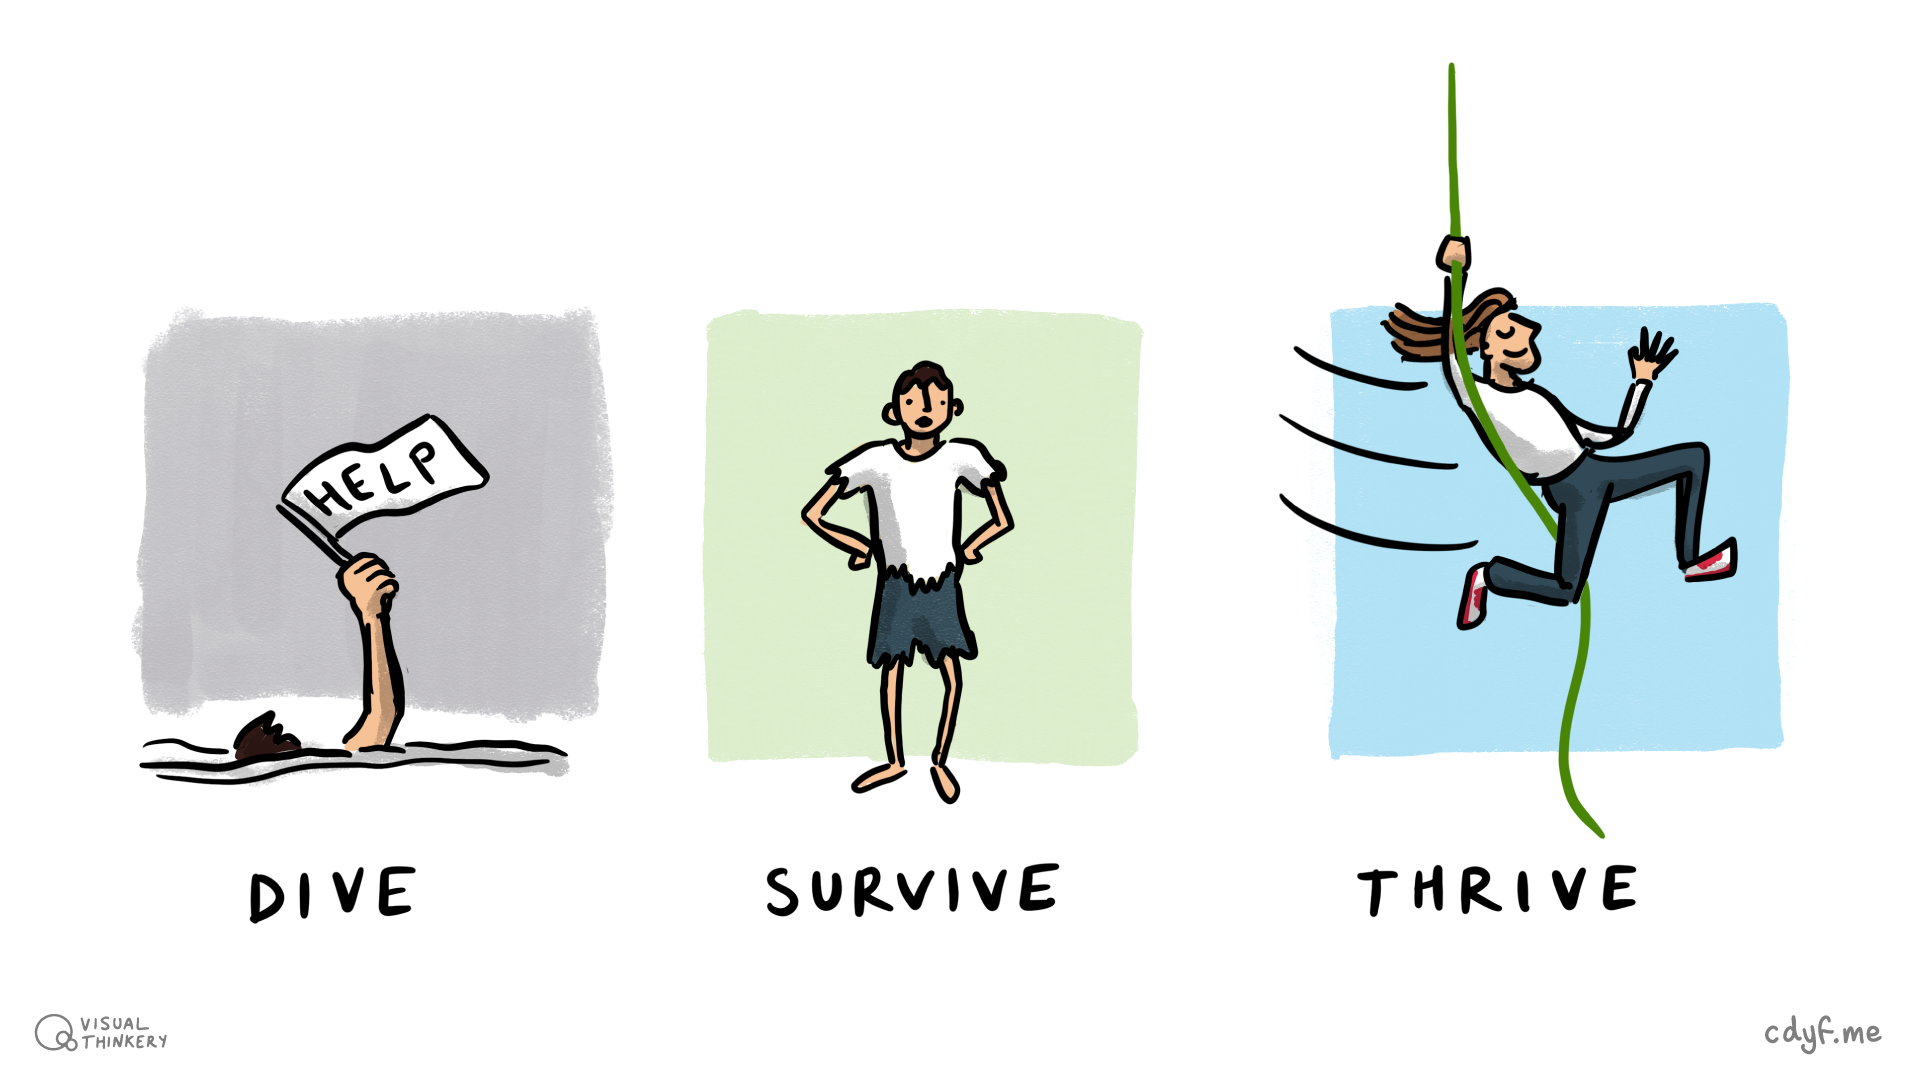
\includegraphics[width=1\linewidth]{images/DiveThriveSurvive} 

}

\caption{How can you survive and thrive on your placement year? Jungle survival sketch by \href{https://visualthinkery.com}{Visual Thinkery} is licensed under \href{https://creativecommons.org/licenses/by-nd/4.0/}{CC-BY-ND}}\label{fig:survival-fig}
\end{figure}



You've done well to find a placement, graduate application ratios hit a record high of \texttt{140:1} this year. \citep{ratio} This confirms what you've probably already found out about the job market being tough for everyone including:

\begin{itemize}
\tightlist
\item
  summer internships
\item
  year long placements
\item
  graduate vacancies
\end{itemize}

So, you've done well to find a placement in a very competitve job market, give yourself a pat on the back!

\section{Key dates}\label{keydates}

Here are a list of all the key dates before, during and after your placement

Obtain and submit plans for formal academic approval deadline, \textbf{31 August 2025}. Once you start your job, there are three key dates, four if you are working outside the UK:

\subsection{First check-in meeting}\label{one}

Initial one-to-one check-in meeting, \textbf{30 September -- 31 October 2025}. Students should coordinate with allocated academic to arrange a suitable time and date.

\subsection{Second check-in meeting}\label{two}

For students on placement outside the UK (only) \textbf{20-31 January 2026} Students should coordinate with allocated academic to arrange a suitable time and date.

\subsection{Manager, Tutor and You meeting}\label{three}

Academic tutor, personal tutor and stuent meeting, \textbf{31 March -- 25 April 2026}. Students should coordinate with academic, supervisor/line manager to arrange a suitable time and date. If you are not able to arrange a date during this time period, the meeting needs to take place before the end of your placement year

\subsection{Project selection}\label{four}

See email from \href{https://research.manchester.ac.uk/en/persons/terence.morley}{Terence Morley}, make your project selections or propose an own project early \textbf{May 2026}

\subsection{Placement report submission}\label{five}

For Bachelors students, your placement report is due at the \textbf{end of welcome week 2026}, submit placement report using the form described in section 6.1

tere

\section{Resitting exams}\label{resits}

If you fail any of your second year exams, you may need to resit them. This doesn't prevent you from doing your placement, but you will need to negotiate some time off to resit any exams and these will need to be done in person in Manchester. \citep{resits}

\chapter{Assessment of your placement year}\label{assessment}

Your placement is formatively assessed, there is no summative assessment. The title ``with industrial experience'' appears in the title of your degree and your degree certicate.

\section{Bachelors degrees: BSc}\label{bsc}

At the end of the year, we ask you to complete a short report using this Microsoft form (UoM login required) \href{https://bit.ly/placement-report-form}{bit.ly/placement-report-form}

As part of that we ask you to complete a skills audit at the beginning and end of the year and compare the results, see \href{https://www.careers.manchester.ac.uk/options/skills/myskills/}{My Skills Development -- on CareerConnect} \citep{audit}

\section{Integrated Masters degrees: MEng}\label{meng}

If you are on the Master of Engineering (MEng) programme, the IE processes are mostly the same as for the BSc programme. The differences are:

\begin{itemize}
\tightlist
\item
  The IE year is taken after year three, not year two
\item
  To stay on the MEng programme you must have a year end average of at least 60\% in years one and two. If you don't, you'll be transferred to the equivalent bachelor's programme. If your year three average is below 60\% you will graduate.
\item
  The Meng students who don't do an IE year will do a short (9 -- 12 week) placement over the summer between years three and four.
\item
  The placement is assessed in COMP40901 by a report you submit at the end of September and a seminar you give during Reading Week. This unit is worth 25 credits of the final year.
\end{itemize}

Speak to the MEng tutor to find out more

\chapter{Tutor meeting guide}\label{tutors}

Information for personal tutors (academic staff) interviewing students (and their managers) on placement.

\section{Purpose of the meeting}\label{purpose}

The purpose of the meeting between you (the tutor), your tutee (the student) and their manager(s) is to:

\begin{enumerate}
\def\labelenumi{\arabic{enumi}.}
\tightlist
\item
  Find out what they have been doing\\
\item
  Get students to reflect on what they've done well, with their manager
\item
  Get students to reflect on what they could do better, with their manager
\item
  Record that the meeting has taken place
\item
  AOB
\end{enumerate}

Most employers can do these visits remotely via Microsoft Teams, Zoom or similar video conferencing software.

Once you've visited your tutees, please fill in the short tutees form at \url{bit.ly/placement-visit-form} (UoM login required) to capture this information and so that we know which students have been visited. The meetings usually last somewhere between 15 and 30 minutes, we've a suggested agenda below.

\section{What have you been doing?}\label{what}

Ask the student to describe what they have been doing since they started on placement and how that fits into the wider organisation they are a part of.

\begin{itemize}
\tightlist
\item
  Tell me about your employerm
\end{itemize}

Most employers can do these visits remotely via Microsoft Teams, Zoom or similar video conferencing software.

\begin{itemize}
\tightlist
\item
  Tell me about your employer and the products or services they provide?
\item
  Which products or services have you been working on?
\item
  What methodologies and tools have you been using?
\item
  What have you been surprised by since you started work?
\end{itemize}

\section{What Went Well (WWW)?}\label{www}

What is going well? Ask the student first, then their manager. Compare results.

\begin{itemize}
\tightlist
\item
  Are there any projects or achievements you are particularly proud of (ask student first, then their manager) compare results
\item
  What skills or knowledge have you managed to build so far, include soft \& hard skills?
\end{itemize}

\section{Even Better If (EBI)?}\label{ebi}

What do they need to improve

\begin{itemize}
\tightlist
\item
  What areas have you identified for improvement in the future (ask student first, then their manager) compare results
\item
  How are you planning to develop these skills? Include soft \& hard skills
\item
  Are there any other things you want to work on before the placement finishes?
\end{itemize}

\section{Any Other Business (AOB)}\label{aob}

This is an opportunity to remind students who don't read their email that:

\begin{itemize}
\tightlist
\item
  They need to choose a 3rd year honours project: This is a good opportunity to check that the student has chosen or proposed a final year project. They've already received information about this from Terence Morley, but it might help to remind them.
\item
  They need to write a placement report:

  \begin{itemize}
  \tightlist
  \item
    For Bachelors students, there's a short placement report form to fill in by September at \href{https://forms.office.com/e/K1gAuWrnex}{forms.office.com/e/K1gAuWrnex} (UoM login required)
  \item
    For MEng students, the details for MEng report submission see COMP40901
  \end{itemize}
\item
  Ask the employer if they are interested in joining our industry club, careers fairs etc record any contact details (names, email addresses) at \url{bit.ly/placement-visit-form}
\end{itemize}

\section{Scheduling meetings using Outlook}\label{schedule}

Students typically finish their placements anytime between June and August, so it's usually best to have the meeting before end of May or early June.

You may find the tools in Outlook useful for scheduling the meeting, there are a few ways of doing this:

\begin{itemize}
\tightlist
\item
  \href{https://outlook.office.com/bookwithme}{outlook.office.com/bookwithme}
\item
  Bookings with me is a service you may need to ask IT services to activate, see \href{https://www.itservices.manchester.ac.uk/ourservices/popular/microsoft365/bookings/}{www.itservices.manchester.ac.uk/ourservices/popular/microsoft365/bookings}
\item
  an alternative is to use a scheduling poll, works on Windows, Mac and the browser version of outlook.office.com \citep{poll}
\end{itemize}

\chapter{Key contacts}\label{contacts}

This page lists contacts that will be useful to you on your placement year

\section{Main contacts}\label{main}

\begin{itemize}
\tightlist
\item
  For academic leads see section \ref{team}
\item
  Computer Science placements team: \href{mailto:CSPlacementsAcademicTeam@manchester.ac.uk}{\nolinkurl{CSPlacementsAcademicTeam@manchester.ac.uk}}
\item
  Engineering placements administration team: \href{mailto:Soe.placements@manchester.ac.uk}{\nolinkurl{Soe.placements@manchester.ac.uk}}
\end{itemize}

\section{Emergency contacts}\label{emergency}

In an emergency if you are a Manchester student working overseas please contact AIG \url{tel:+441273552922} or \href{mailto:CorporateAssist@aig.com}{\nolinkurl{CorporateAssist@aig.com}}

The University operate a 24 hour emergency helpline \url{tel:+441613069966}

Whilst on placement the responsibility for looking after your health and safety rests with your employer.

Students should raise any concerns in the first place with the workplace supervisor (your manager) and then either through the management line of with the Health \& Safety contact. If issues are not resolved, then you should contact the placement academic or placements team \href{mailto:soe.placements@manchester.ac.uk}{\nolinkurl{soe.placements@manchester.ac.uk}}.

\section{Careers service}\label{careers}

The Careers Service offers support and advice throughout your time at the University of Manchester to help you make the most of your time here and best prepare you for your future. They can also advise you about your placement and career plans, see \href{https://www.careers.manchester.ac.uk/}{www.careers.manchester.ac.uk/}

\section{Wellbeing Support Services}\label{wellbeing}

Wellbeing Support Services, see \url{https://www.studentsupport.manchester.ac.uk/taking-care/} \citep{wellbeing}

TODO:

\section{Disability Advisory and Support Service: DASS}\label{dass}

DASS provides equity of services to everyone regardless of people's age, disability, gender, gender
identity, race, religion or belief or sexual orientation.

TODO: finish

  \bibliography{book.bib}

\end{document}
